\documentclass[12pt, a4paper]{article}

%====================== PACKAGES ======================
\usepackage{extsizes}
% \usepackage[french]{babel}
\usepackage[utf8x]{inputenc}
\usepackage{hyperref}
\usepackage{multicol}
\usepackage[scale=0.8]{geometry}
% \usepackage{fontspec}
\usepackage{tkz-graph}
\usepackage{pgf,tikz}
\usepackage{graphicx}
\usepackage{eurosym}
\usepackage{float}

\newenvironment{Figure}
  {\par\medskip\noindent\minipage{\linewidth}}
  {\endminipage\par\medskip}

\renewcommand{\baselinestretch}{1.25} 
\usepackage{mathrsfs}\usetikzlibrary{arrows}
\usepackage{caption}

\hypersetup{
    % bookmarks=true,         % show bookmarks bar?
    unicode=false,          % non-Latin characters in Acrobat’s bookmarks
    pdftoolbar=true,        % show Acrobat’s toolbar?
    pdfmenubar=true,        % show Acrobat’s menu?
    pdffitwindow=false,     % window fit to page when opened
    pdfstartview={FitH},    % fits the width of the page to the window
    pdftitle={Rapport},    % title
    pdfauthor={Loris},     % author
    pdfsubject={Prepro},   % subject of the document
    pdfcreator={},   % creator of the document
    pdfproducer={}, % producer of the document
    pdfkeywords={}, % list of keywords
    pdfnewwindow=true,      % links in new PDF window
    colorlinks=true,       % false: boxed links; true: colored links
    linkcolor=black,          % color of internal links (change box color with linkbordercolor)
    linkbordercolor=white,
    citecolor=green,        % color of links to bibliography
    filecolor=magenta,      % color of file links
    urlcolor=cyan           % color of external links
}

\usepackage[T1]{fontenc}
\usepackage{multicol}

\author{Elouan \textsc{Lebaillif} \and Jordan \textsc{Daffix} \and Loris \textsc{Croce}}

\title{\rule{\textwidth}{1pt} \\ \Huge\textbf{IT Sounds cool: } \\ \emph{English L3} \rule{\textwidth}{1pt}}

\begin{document}

\begin{titlepage}
    \centering
    \vfill
    {
      \rule{\textwidth}{1pt} \\ 
      \Huge\textbf{Project report} \\ 
      \emph{English L3} \rule{\textwidth}{1pt}
    
\includegraphics[width=10cm]{pictures/Logo.png} % also works with logo.pdf
      \vfill
      {
        \small
        Elouan \textsc{Lebaillif} \ \ Jordan \textsc{Daffix} \ \ Loris \textsc{Croce}
      }
    }
    \vfill
    
\includegraphics[width=3cm]{pictures/Logo-UCA.png} % also works with logo.pdf
    \vfill
    \vfill
    \vfill
\end{titlepage}

% \maketitle{}

\tableofcontents

\newpage

\section{Introduction}

We are Jordan, Loris and Elouan, students in the third degree in Computer Sciences, at the University Clermont Auvergne.

\paragraph{Why this project}
We all dream of calm. Of peace. It is with this main idea that the project of \emph{I.T. Sounds Cool} was born. Our best engineers then worked to create the perfect product for everyone to get the tranquility they deserve: a parametrable anti-noise headset that can adapt to all situations of everyday life.

\section{Organization}

\subsection{Timeline}

\begin{table}[!h]
\centering
\caption{Timeline}
\label{my-label}
\begin{tabular}{|l|c|c|c|c|c|c|c|c|}
\hline
\textbf{TASKS / WEEKS} & \textit{\textbf{1}} & \textit{\textbf{2}} & \textit{\textbf{3}} & \textit{\textbf{4}} & \textit{\textbf{5}} & \textit{\textbf{6}} & \textit{\textbf{8}} & \textit{\textbf{9}} \\ \hline
\textbf{Conceptions of the product} & 1h30 & 1h30 & 30mn & 30mn & 1h & 1h &  &  \\ \hline
\textbf{Search videos} &  & 1h & 1h & 2h & 20mn & 1h &  & 1h \\ \hline
\textbf{Report} &  &  &  & 30mn & 10mn & 1h & 1h & 5h \\ \hline
\textbf{Trailer (storyboard + montage)} &  &  &  & 2h & 1h30 &  & 30mn & 5h \\ \hline
\end{tabular}
\end{table}

\subsection{Role of each team member}

\begin{itemize}

    \item Report: 
        \begin{itemize}
        \item Writing: everyone
        \item Layout: Loris
        \end{itemize}
    \item Video search: everyone
    \item Storyboard and montage of the trailer: Jordan
    \item Images of application: Jordan
    \item Idea : Jordan
    \item Logo: Jordan
    \item Model: Elouan

\end{itemize}

\section{Description of the product}

    \subsection{Technical description}

    Our device takes from as an headset that is equipped with microphones and speakers. On the inside there's a chipset in charge of interpretating commands from the the application in order to filter sounds. Like annoying noises, It analyzes the different frequencies to mute those you don't want.

    \begin{figure}[!h]
        \centering
        \definecolor{ccqqqq}{rgb}{0.8,0,0}\definecolor{qqccqq}{rgb}{0,0.8,0}\definecolor{qqqqff}{rgb}{0,0,1}\definecolor{cqcqcq}{rgb}{0.7529411764705882,0.7529411764705882,0.7529411764705882}
        \begin{tikzpicture}[line cap=round,line join=round,>=triangle 45,x=1cm,y=1cm]\draw [color=cqcqcq,, xstep=0.5cm,ystep=0.5cm] (-0.4774576901689461,-1.177409646121973) grid (8.854989703419555,5.305051889578338);\clip(-0.4774576901689461,-1.177409646121973) rectangle (8.854989703419555,5.305051889578338);\draw[line width=1pt,color=qqqqff,smooth,samples=100,domain=-0.4774576901689461:8.854989703419555] plot(\x,{sin(((\x))*180/pi)});\draw[line width=1pt,color=qqccqq,smooth,samples=100,domain=-0.4774576901689461:8.854989703419555] plot(\x,{2+sin(((\x)*2)*180/pi)});\draw[line width=1pt,color=ccqqqq,smooth,samples=100,domain=-0.4774576901689461:8.854989703419555] plot(\x,{4+sin(((\x)*4)*180/pi)});\end{tikzpicture}
        \caption{Examples of high medium and low frequencies (from up to down)}
    \end{figure}

    \begin{figure}[!h]
        \centering
        \definecolor{dtsfsf}{rgb}{0.8274509803921568,0.1843137254901961,0.1843137254901961}\definecolor{qqqqff}{rgb}{0,0,1}\definecolor{cqcqcq}{rgb}{0.7529411764705882,0.7529411764705882,0.7529411764705882}\begin{tikzpicture}[line cap=round,line join=round,>=triangle 45,x=5cm,y=5cm]\draw [color=cqcqcq,, xstep=0.1cm,ystep=0.1cm] (-0.2708819694654514,-0.7261888854321853) grid (1.8119632309392317,0.7205874345412162);\draw[->,color=black] (-0.2708819694654514,0) -- (1.8119632309392317,0);\foreach \x in {-0.2,0.2,0.3,0.4,0.5,0.6,0.7,0.8,0.9,1,1.1,1.2,1.3,1.4,1.5,1.6,1.7,1.8}\draw[shift={(\x,0)},color=black] (0pt,2pt) -- (0pt,-2pt) node[below] {\footnotesize $\x$};\draw[->,color=black] (0,-0.7261888854321853) -- (0,0.7205874345412162);\foreach \y in {-0.7,-0.6,-0.5,-0.4,-0.3,-0.2,-0.1,0.2,0.3,0.4,0.5,0.6,0.7}\draw[shift={(0,\y)},color=black] (2pt,0pt) -- (-2pt,0pt) node[left] {\footnotesize $\y$};\draw[color=black] (0pt,-10pt) node[right] {\footnotesize $0$};\clip(-0.2708819694654514,-0.7261888854321853) rectangle (1.8119632309392317,0.7205874345412162);\draw[line width=1pt,color=qqqqff,smooth,samples=100,domain=-0.2708819694654514:1.8119632309392317] plot(\x,{0.5*cos(((\x)*5)*180/pi)});\draw[line width=1pt,color=dtsfsf,smooth,samples=100,domain=-0.2708819694654514:1.8119632309392317] plot(\x,{0.5*cos((3.1415926535+(\x)*5)*180/pi)});\end{tikzpicture}
        \caption{Example of \emph{phase opposition}, phenomenom used to bypass sounds}
    \end{figure}

    \newpage

    \subsection{Physical description}

    \emph{I.T. sounds cool\textsuperscript{TM}}'s device can take shape of headphones or headsets, depending preferences of the customers. Its weight is about $320g$ and its battery life (in use) is $48 h$.

    \begin{multicols}{2}
        \begin{Figure}
        \centering
        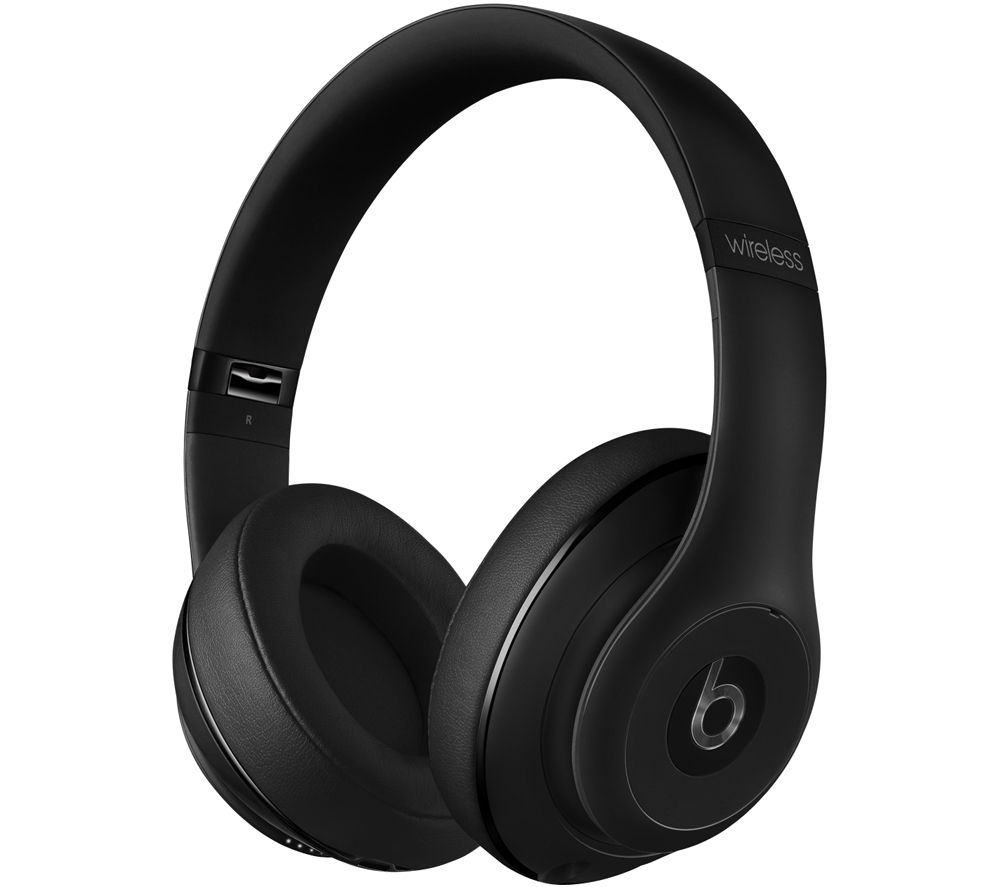
\includegraphics[width=5cm]{pictures/casque1.png}
        \end{Figure}
        \begin{Figure}
        \centering
        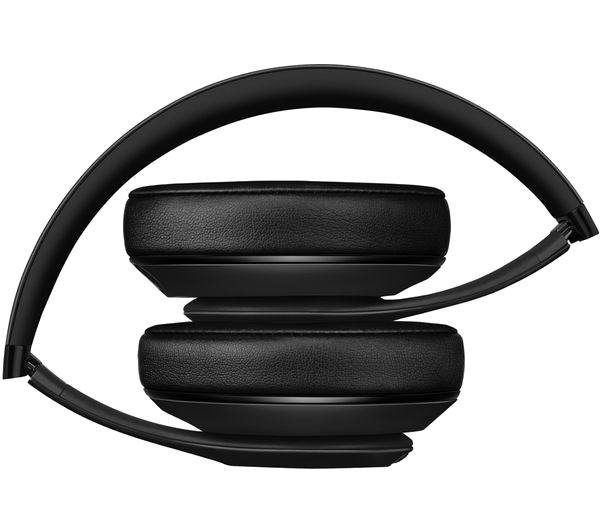
\includegraphics[width=5cm]{pictures/casque2.png}
        \end{Figure}
    \end{multicols}

    The price of the product would be approximatively of 299\EUR , depending the model. It would first be producted in small quantities in order to test the marketshare. As it's important for us we would like to provide the lowest ecological cost for the production of this product by prefering short transfer circuit and recyclable materials.

    \paragraph{Further details}
    \begin{itemize}
        \item Synthetic leather look ear pieces.
        \item 1.2m cord length.
        \item Adjustable headband.
        \item 3.5mm jack
        \item 40mm driver.
        \item Manufacturer's 2 year guarantee.
        \item The headset comes with a code to access the application.
    \end{itemize}

    \begin{figure}[h]
        \centering
        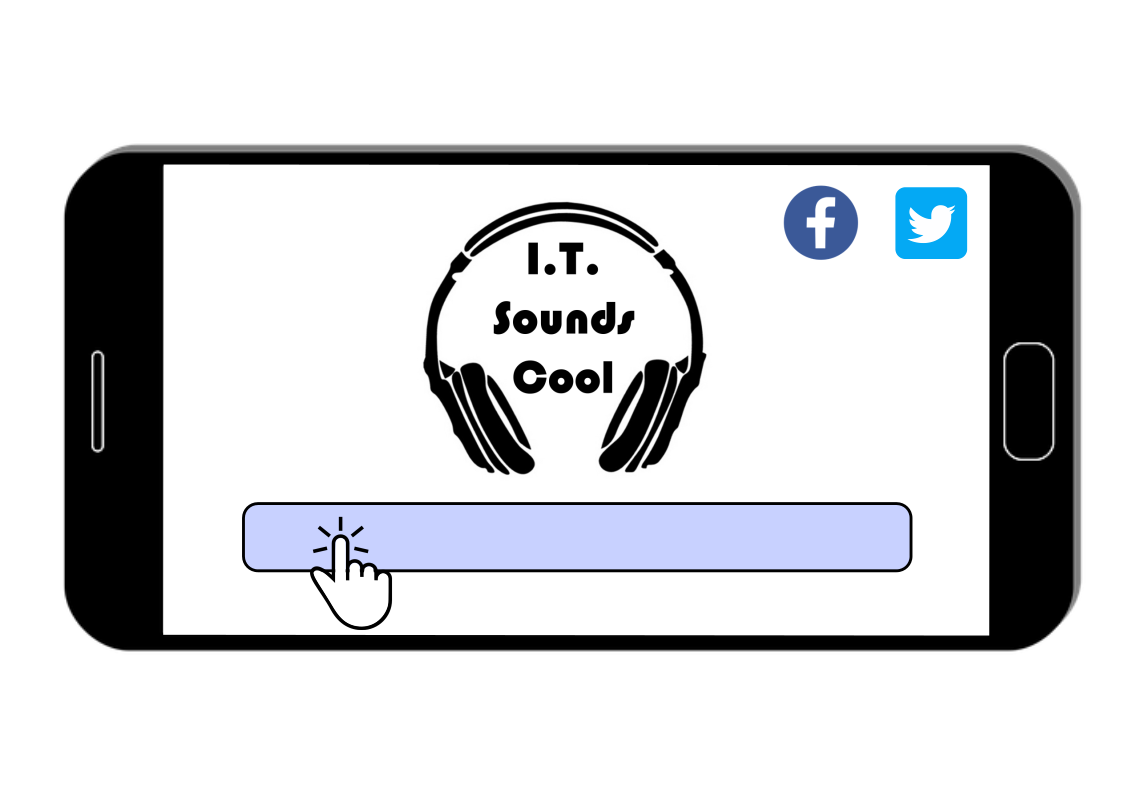
\includegraphics[width=5cm]{pictures/AppSoundsCoolMenu.png}
    \end{figure}

    \subsection{Functional description}

    The device itself is connected to a dedicated mobile application that allows to monitor it. It's also possible to get filtering presets and customize them. The microphones receive frequencies from ambient sound and analyse it in real time to \emph{dephase} selected frequencies.

    \begin{figure}[h]
        \centering
        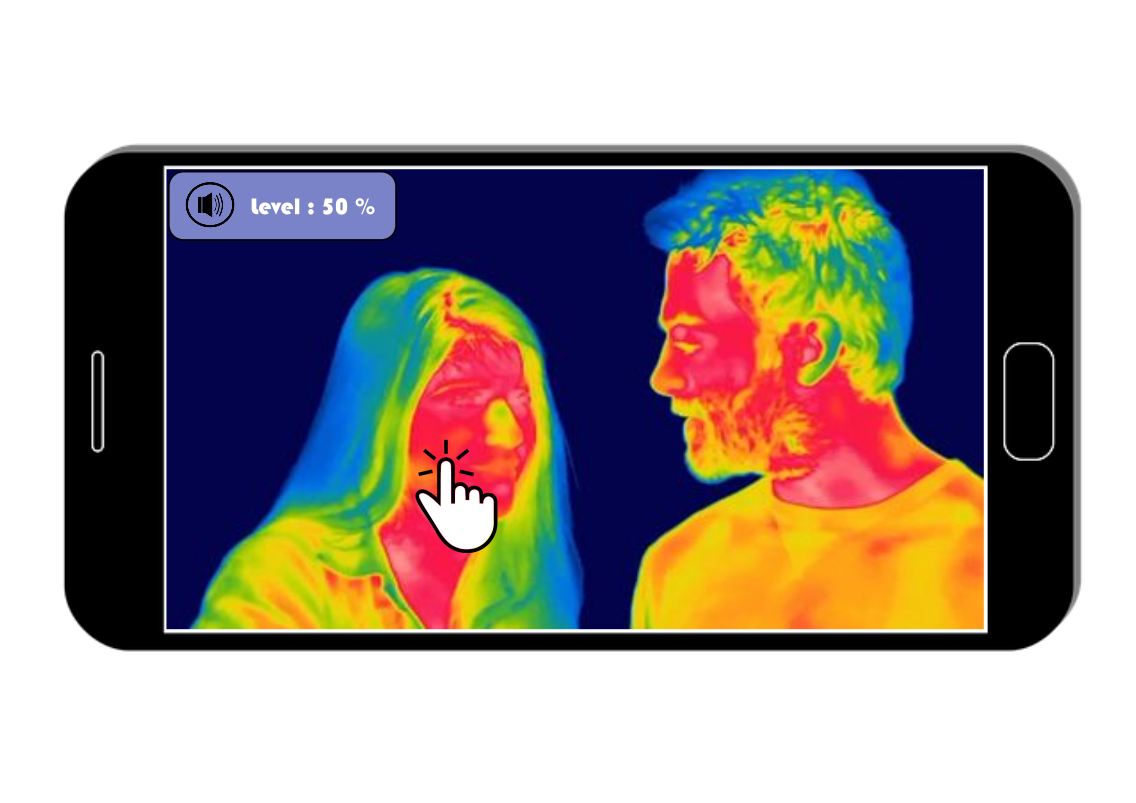
\includegraphics[width=8cm]{pictures/AppSoundsCool.png}
        \caption{Sound filtering prototype}
    \end{figure}

    Look at this happy couple who declare themselves their flame. Like any normal embittered person, it annoys you - and who would not be disturbed ? Our app can detect surrounding sound frequencies and give you a clear view of your environment. All you have to do is select the noisomes and adjust the settings. For example, you can lower the sound or completely mute the sound source.

    You also have access to a list of presets that will allow you to eliminate some noisomes automatically. Frequent updates are made and you can download new packages from our website:
    
    \url{http://www.itsoundscool.com}

    \begin{multicols}{2}
        \begin{Figure}
        \centering
        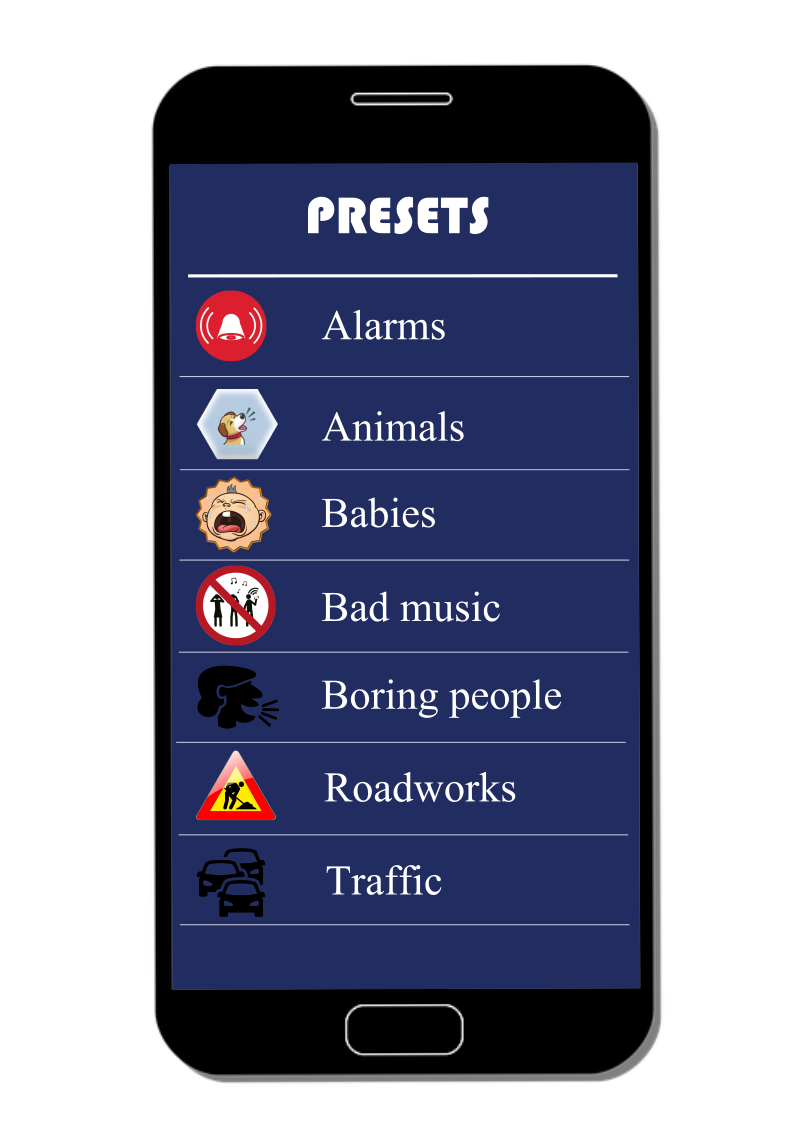
\includegraphics[width=5cm]{pictures/AppSoundsCoolPresets.png}
        \end{Figure}

        The results collected by our current customers are edifying: hearing loss, headaches and depression have dropped drastically, so as symptoms of agoraphobia in public transit. Everyone praised well-being restored, more restful sleep and a feeling of finding oneself.

    \end{multicols}

    % \begin{figure}[!h]
    %     \centering
    %     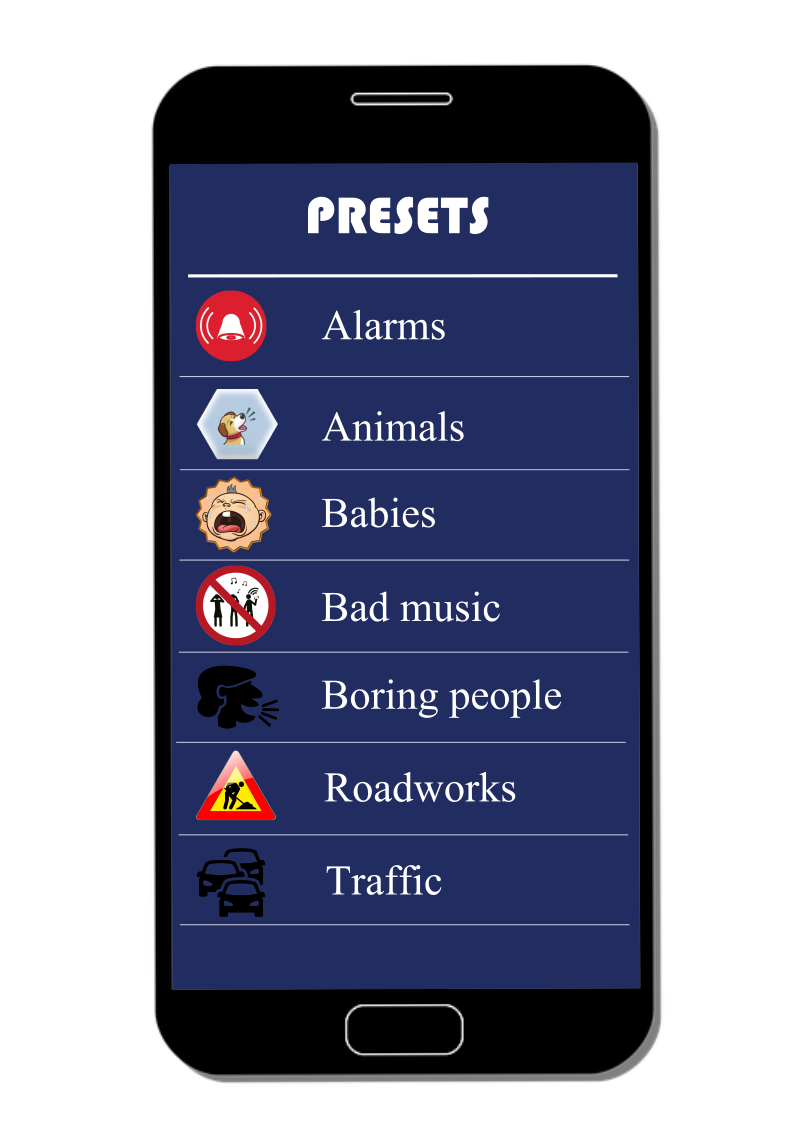
\includegraphics[width=5cm]{pictures/AppSoundsCoolPresets.png}
    %     \caption{Presets prototype }
    % \end{figure}

    % The results collected by our current customers are edifying: hearing loss, headaches and depression have dropped drastically, so as symptoms of agoraphobia in public transit. Everyone praised well-being restored, more restful sleep and a feeling of finding oneself.

    \begin{figure}[!h]
        \centering
        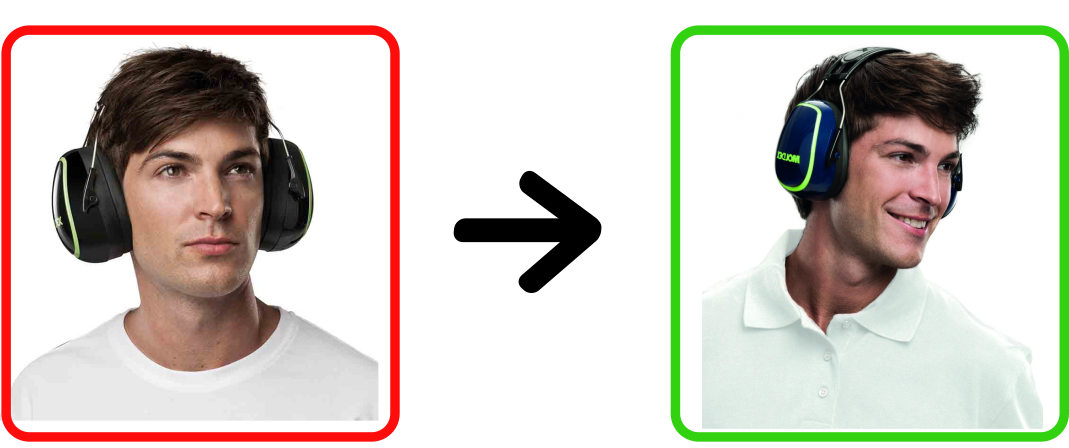
\includegraphics[width=10cm]{pictures/AppHappy.png}
        \caption{Headphones prototype}
    \end{figure}

    However, we must make it clear to our customers that wearing too much noise-cancelling headphones may cause the notes to drop if it is used in class and a lack of sociability, or even the loss of your friends if they catch you. To allow more discretion, we are working on another undetectable product: the bluetooth earphone - which will soon be on sale.

    % \newpage

    \section{Storyboard}

    \begin{flushleft}
    \fontfamily{lmtt}\selectfont

    \emph{\textbf{Heavenly place}}\medskip

    We all dream of peace. Of Calmness. And freedom.\medskip

    \emph{\textbf{Storm and related shots}}\medskip

    But dark clouds prevent each of us from reaching inner peace. The annoying sound sources come from everywhere. It can be the neighbor's dog while you're trying to sleep. The so-called cute crying baby you want to murder. The boring teacher who saves you money on sleeping pills. Your dear friend much too talkative.The man with tics, and the one who listens to bad music and thinks he's alone in the subway.\medskip

    \emph{\textbf{Expert speaking}}\medskip

    There are so many causes that can have a fundamental impact on our well-being.\medskip

    \emph{\textbf{Scientists working}}\medskip

    That's why our best engineers worked to create the perfect product for everyone to get the tranquility they deserve: a parametrable anti-noise headset that can adapt to all situations of everyday life.\medskip

    \emph{\textbf{People with headphones and smartphones}}\medskip

    From your smartphone, you can select the surrounding harmful sound sources and adjust their level. You also have access to a series of presets updated regularly. You just need to don your headset, and enjoy the quietness.\medskip

    \emph{\textbf{Relaxed people}}\medskip

    No more uncomfortable noises. No more headaches. You are the total master of your ears. You are free and can finally have access to your inner peace.\medskip
    \end{flushleft}  

    \fontfamily{lmr}\selectfont

    \section{Individual reflection}

    \paragraph{Jordan}

    \begin{quotation}
    \emph{This project allowed me to get skills on topics that I would not necessarily be interested in.
    Indeed, I learnt to make a video montage and photo montages, and I was able to unleash my creativity trying to find fun ideas. Of course all of this was very time-consuming, but it also was entertaining and informative - although it does not necessarily have to do with English!
    I was also able to improve my teamwork because we were a group of three and we had to share the tasks to work effectively.
    Finally, I could improve my knowledge of English by doing research on the Internet to find all kinds of ideas for our project. I also worked on my pronunciation to have a correct rendering of the trailer - and to be not too ashamed.}
    \end{quotation}

    \paragraph{Loris}

    \begin{quotation}
    \emph{Thanks to this project I made discoveries on a part of technology who is really rewarding and to me part of a close future. To be honest, this is aproduct which I dreamed about in many situations, because I'm really obessed by noises and lived in some noisy places. On a more project-oriented side, this one was very challenging, knowing that there is already some less efficient but related products. Hopefully we already worked together as a team and I think it was our strentgh since we have different skills and sensitivities.}
    \end{quotation}

    \paragraph{Elouan}

    \begin{quotation}
    \emph{To me, this project was really interesting in many different ways. First, I made a lot of researches about ears and sounds, which was a subject I never even worried about. It was also great to work with Loris and Jordan with whom I already worked on a project. We already knew each other so we directly worked on the project. The funny thing is to think about a project which is realizable and that had never been done before, this was the hard part of the job. 
    Then trying to find a cool name for the project and everything makes me wonder if we made an english project or a true project!}
    \end{quotation}

    \section{Webography}

    \begin{itemize}
    \item \url{https://www.shutterstock.com/}
    \item \url{http://dictionnaire.reverso.net/}
    \item \url{https://electronics.howstuffworks.com}
    \item \url{https://en.wikipedia.org/wiki/Reflection_phase_change}
    \end{itemize}

% Pas oublier pages perso

\end{document}